\section{Aufbau von M$^2$etis}
\label{chap:grundlagen:aufbau_metis}

Diese Arbeit entsteht im Rahmen des \ac{m2etis}-Projektes Cite Cite Cite und bla.

\begin{figure}[htbp]
\centering
\resizebox{\textwidth}{!}{%
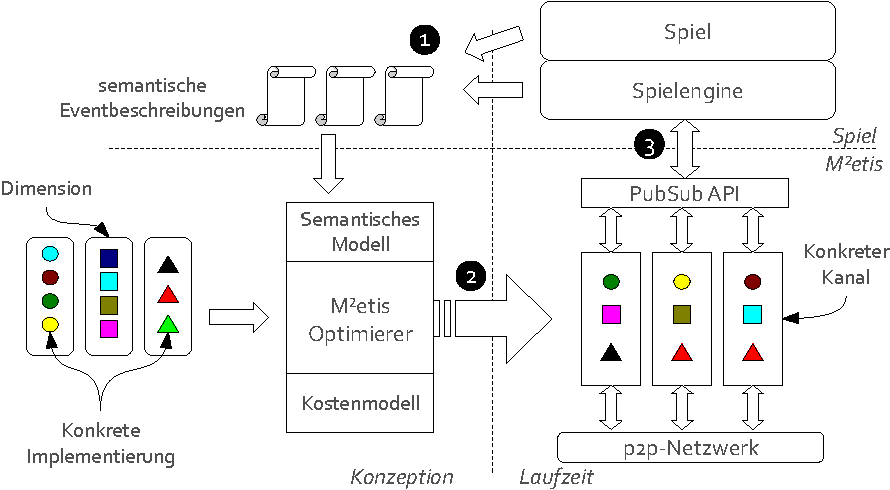
\includegraphics{grafics/metis_aufbau.pdf}}
\caption{Architekturübersicht von \ac{m2etis}}
\label{fig:metis_aufbau}
\end{figure}

\cite{Fischer2010a, Fischer2010Event}

